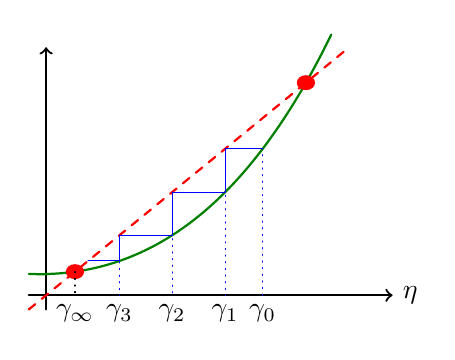
\begin{tikzpicture}[line cap=round, line join=round, xscale=11, yscale=9]

  % 1. Axes
  \draw[->,thick] (-0.02,0) -- (0.4,0) node[right] {$\eta$};
  \draw[->,thick] (0,-0.02) -- (0,0.35) node[above] {};

  % 2. Red diagonal y = x
  \draw[red,thick,dashed,samples=200,domain=-0.02:0.35]
       plot(\x,\x);

  % 3. Green curve 
  \draw[Green,thick,samples=200,domain=-0.02:0.33]
       plot(\x,{(2*(\x)^2 + 0.03)/(1-\x)});

  \coordinate (Xinf)  at (0.033333, 0.033333);
  \coordinate (Xzero) at (0.3, 0.3);


  \fill[red] (Xinf) circle(0.3pt);
  \fill[red] (Xzero) circle(0.3pt);

  \draw[dotted,black] (Xinf) -- (Xinf|-0,0);
  
  \coordinate (eta0) at (0.25, 0);
  \node[black,below] at (eta0) {$\gamma_0$};
  \coordinate (f1eta0) at (0.25, 0.206667);
  \draw[dotted,blue] (eta0) -- (f1eta0);
  \coordinate (eta1) at (0.206667,0.206667);
  \draw[solid,blue] (f1eta0) -- (eta1);
  \coordinate (f1eta1) at (0.206667, 0.145491);
  \draw[solid,blue] (eta1) -- (f1eta1);
  \node[black,below] at (eta1|-0,0){$\gamma_1$};
  \draw[dotted,blue] (eta1) -- (eta1|-0,0);
  \coordinate (eta2) at (0.145491,0.145491);
  \node[black,below] at (eta2|-0,0){$\gamma_2$};
  \draw[dotted,blue] (eta2) -- (eta2|-0,0);
  \draw[solid,blue] (f1eta1) -- (eta2);
  \coordinate (f1eta2) at (0.145491, 0.084651);
  \draw[solid,blue] (eta2) -- (f1eta2);
  \coordinate (eta3) at (0.084651,0.084651);
  \node[black,below] at (eta3|-0,0){$\gamma_3$};
  \draw[dotted,blue] (eta3) -- (eta3|-0,0);
  \draw[solid,blue] (f1eta2) -- (eta3);
  \coordinate (f1eta3) at (0.084651, 0.048431);
  \draw[solid,blue] (eta3) -- (f1eta3);
  \coordinate (eta4) at (0.048431,0.048431);
  \draw[solid,blue] (f1eta3) -- (eta4);

  \node[black,below] at (Xinf|-0,0) {$\gamma_\infty$};
  %\node[black,below] at (Xzero|-0,0) {$\gamma_{0}$};

\end{tikzpicture}